%% The first command in your LaTeX source must be the \documentclass command.
%%
%% Options:
%% twocolumn : Two column layout.
%% hf: enable header and footer.
\documentclass[
% twocolumn,
% hf,
]{ceurart}

%%
%% One can fix some overfulls
\sloppy

%%
%% Minted listings support 
%% Need pygment <http://pygments.org/> <http://pypi.python.org/pypi/Pygments>
\usepackage{listings}
%% auto break lines
\lstset{breaklines=true}


%%
%% DL Logo for inline use
\usepackage{graphbox}
\DeclareRobustCommand{\DLLogo}{%
  \begingroup\normalfont
  \kern-1.75pt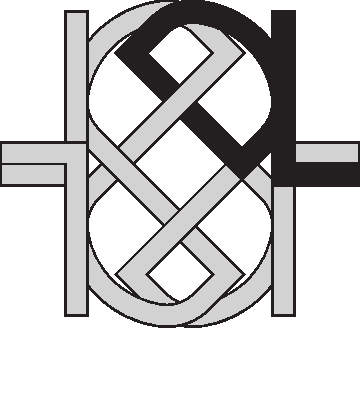
\includegraphics[align=c,height=1.25\baselineskip]{dl}\kern-1.5pt%
  \endgroup
}

%%
%% AMS Theorems
\usepackage{amsthm}
\newtheorem{theorem}{Theorem}
\newtheorem{definition}{Definition}
\newtheorem{example}{Example}


%%%%%%%%%%%%%%%%%%%%%%%%%%%%%%%%%%%%%%%%
%%% OUR SETTINGS
\usepackage{amsmath}
\usepackage{amssymb}
\usepackage{mathtools}
\usepackage{algorithm}
\usepackage{algpseudocode}
% \usepackage{theorem}
\usepackage{xspace}
\usepackage{dl}
\usepackage{url}
%\usepackage[numbers]{natbib}
\clubpenalty = 10000
\widowpenalty = 10000
\displaywidowpenalty = 10000
% theorems and the like
% \newtheorem{theorem}{Theorem}
\newtheorem{lemma}{Lemma}
% \newtheorem{proposition}{Proposition}
% \newtheorem{corollary}{Corollary}

% \theorembodyfont{\rmfamily}
% \newtheorem{definition}{Definition}
% \newtheorem{example}{Example}

% \theorembodyfont{\slshape}
% \newtheorem{assumption}{Assumption}

% \theorembodyfont{\slshape}
% \newtheorem{hypothesis}{Hypothesis}

% \newenvironment{justification}{\textsf{Justification:}}{\hfill $\Box$}
%\newenvironment{proof}{\noindent\textsc{proof:}}{\hfill $\square$ \bigskip}


\newcommand{\AL}{\ensuremath{\mathcal{AL}}\xspace}
\newcommand{\ALC}{\ensuremath{\mathcal{ALC}}\xspace}
\newcommand{\SROIQ}{\ensuremath{\mathcal{SROIQ}}\xspace}
\newcommand{\onto}[1]{\ensuremath{\mathsf{#1}}}
\usepackage[colorinlistoftodos]{todonotes}

\newcommand{\cg}
{\ensuremath{\blacktriangle}\xspace}
%{\ensuremath{\dot{\sqcup}}\xspace}

\newcommand{\todoT}[1]{\todo[fancyline,size=\small,color=orange!40]{\textbf{TBD:} #1}\xspace}
\newcommand{\todoR}[1]{\todo[fancyline,size=\small,color=orange!40]{\textbf{rc:} #1}\xspace}

\newcommand{\todoO}[1]{\todo[fancyline,size=\small,color=red!20]{\textbf{ok:} #1}\xspace}

\newcommand{\tododo}[1]{\todo[fancyline,size=\small,color=red!60]{\textbf{ToDO:} #1}\xspace}
\newcommand{\todoin}[1]{\todo[inline,size=\small,color=green!20]{\textbf{HERE:} #1}\xspace}


%\usepackage{pgf}https://preview.overleaf.com/public/pqghhhhwjqpw/images/986e3685291cb332a5fbe5a979b5045d2e649a43.jpeg
\usepackage{tikz}
%\usetikzlibrary{arrows,automata}
\usetikzlibrary{positioning,calc,backgrounds}

%%%%%%%MACROS%%%%%%%%
\newcommand{\Imc}{\ensuremath{\mathcal{I}}\xspace}
\newcommand{\Jmc}{\ensuremath{\mathcal{J}}\xspace}
\newcommand{\Tmc}{\ensuremath{\mathcal{T}}\xspace}
\newcommand{\Amc}{\ensuremath{\mathcal{A}}\xspace}
\newcommand{\Rmc}{\ensuremath{\mathcal{R}}\xspace}
\newcommand{\Omc}{\ensuremath{\mathcal{O}}\xspace}
\newcommand{\Omcref}{\ensuremath{\mathcal{O}_\mathrm{ref}}\xspace}
\newcommand{\Omcfull}{\ensuremath{\mathcal{O}_\mathrm{full}}\xspace}
\newcommand{\Ontology}{\Omc}

% \newcommand{\sub}{\ensuremath{\mathsf{sub}}\xspace}
\newcommand{\subr}{\ensuremath{\mathsf{subr}}\xspace}

\newcommand{\EL}{\ensuremath{\mathcal{E\!L}}\xspace}
\newcommand{\elpp}{\ensuremath{\mathcal{E\!L}^{++}}\xspace}
% \newcommand{\DL}{{\ensuremath{\mathcal{DL}}}\xspace}

\newcommand{\Inf}{{\ensuremath{\mathsf{Inf}}}\xspace}
\newcommand{\qual}{{\ensuremath{\mathsf{IIC}}}\xspace}

\newcommand{\Tup}{{\ensuremath{\mathsf{UpCover}_\Ontology}}\xspace}
\newcommand{\Tdown}{{\ensuremath{\mathsf{DownCover}_\Ontology}}\xspace}
\newcommand{\gammaT}{{\ensuremath{\gamma_\mathcal{T}}}\xspace}
\newcommand{\rhoT}{{\ensuremath{\rho_\mathcal{T}}}\xspace}
%\newcommand{\gammaT}{{\ensuremath{\gamma_{\mathcal{T}}}\xspace}
%\newcommand{\rhoT}{{\ensuremath{\rho_{\mathcal{T}}}\xspace}

\newcommand{\disjoint}{\ensuremath{\mathit{disjoint}}\xspace}
\newcommand{\self}{\ensuremath{\mathit{Self}}\xspace}
\newcommand{\less}[2]{\ensuremath{\leq #1~#2}\xspace}
\newcommand{\more}[2]{\ensuremath{\geq #1~#2}\xspace}
\newcommand{\nominal}[1]{\ensuremath{\{#1\}}\xspace}

\newcommand{\inv}{\ensuremath{\mathit{inv}}\xspace}
\newcommand{\refine}{\ensuremath{\mathop{\uparrow}}\xspace}
\newcommand{\corefine}{\ensuremath{\mathop{\downarrow}}\xspace}
%\DeclareMathOperator*{\argmax}{\mathsf{arg\,max}}
\DeclareMathOperator*{\argmax}{\mathsf{argmax}}

%%%%%%%%%%%%%%%%%%%%%%%%%%%%%%%%%%%%%%%%




%%
%% end of the preamble, start of the body of the document source.
\begin{document}

%%
%% Rights management information.
%% CC-BY is default license.
\copyrightyear{2023}
\copyrightclause{Copyright for this paper by its authors.
  Use permitted under Creative Commons License Attribution 4.0
  International (CC BY 4.0).}

%%
%% This command is for the conference information
\conference{\DLLogo{} DL 2023: 36th International Workshop on Description Logics,
  September 2--4, 2023, Rhodes, Greece}

%%
%% The "title" command
\title{Implementing Axiom Weakening for SROIQ}

%%
%% The "author" command and its associated commands are used to define
%% the authors and their affiliations.

\author[1]{Roland Bernard}[
email=roland.bernard@student.unibz.it,
]
\author[1]{Oliver Kutz}[
email=oliver.kutz@unibz.it,
]
\author[1]{Nicolas Troquard}[
email=nicolas.troquard@unibz.it,
]
\address[1]{
Free University of Bozen-Bolzano, Italy
}



%%
%% The abstract is a short summary of the work to be presented in the
%% article.
\begin{abstract}
Axiom weakening is a technique that allows for a fine-grained repair of inconsistent ontologies. Its main advantage is that it repairs ontologies by making axioms
less restrictive rather than by deleting them, employing refinement operators.  In this paper, we build on previously introduced axiom weakening for \ALC, and show how it can be extended to deal with \SROIQ, the expressive and decidable description logic underlying OWL 2 DL. 
We here focus on describing a prototype implementation computing axiom weakening for \SROIQ and discuss a number of performance and evaluation aspects. 
%the definitions of the refinement operators to deal with \SROIQ constructs, in particular with %such as reflexive and irreflexive roles, disjoint roles, 
%role hierarchies,  cardinality constraints and nominals, and illustrate its application. Finally, we discuss the problem of termination of an iterated weakening procedure. 
\end{abstract}

%%
%% Keywords. The author(s) should pick words that accurately describe
%% the work being presented. Separate the keywords with commas.
\begin{keywords}
  Description Logic \sep
  Knowledge refinement \sep
  Prot\'eg\'e
\end{keywords}

%%
%% This command processes the author and affiliation and title
%% information and builds the first part of the formatted document.
\maketitle



\section{Introduction: Weakening for debugging}

\section{Axiom Weakening for \ALC}

\section{Extending Weakening to \SROIQ}
\begin{example}
    Some examples for some \SROIQ features.
\end{example}

\section{Implementing Axiom Weakening for \SROIQ}

\section{Weakening makes you strong: evaluation aspects}



%%
%% Define the bibliography file to be used
\bibliography{biblio}

%%
%% If your work has an appendix, this is the place to put it.
\appendix

\section{Introduction}

%TO DOs

%\begin{itemize}
 %   \item Extend Axiom Weakening to \SROIQ. I.e. extend generalisation and specialisation operators to:
  %  \begin{itemize}
   %     \item Cardinality restrictions
    %    \item Role inclusions
     %   \item Nominals
      %  '\item Universal role... 
       % \item reflexive, irreflexive, disjoint roles, these can only be dropped
%    \end{itemize}
    
 %   \item Discuss termination
  %  \item Complexity of axiom weakening for rich DL?
   % '\item Nice examples
%\end{itemize}
%\todoT{Motivating ontology repair, G's examples, overview of other approaches, and our approach.}
The traditional approach to repairing inconsistent ontologies amounts to identify problematic axioms and to remove them (e.g.,~\cite{ScCo03,kalyanpur2005debugging,kalyanpur2006repairing,BaPS07}). Whilst this approach is sufficient to guarantee that the obtained ontology is consistent, it tends to lead to information loss as a secondary effect. For instance, let us assume that our ontology contains the following axioms:
%
\begin{align}
\label{ex:pp2mp}
\con{Polygamist} & \sqsubseteq \con{Person} \;\sqcap \more 2 {\role{married}}.\con{Person}\\
\label{ex:pmp}
\con{Polygamist} & \sqsubseteq \con{MarriedPerson}\\
\label{ex:mpp1mp1mp}
\con{MarriedPerson} & \sqsubseteq \con{Person} \;\sqcap \less 1  {\role{married}}.\con{Person} \;\sqcap \more 1 {\role{married}}.\con{Person}\\
\label{ex:pmary}
\con{Polygamist}(mary) &
\end{align}
%\todoT{Maybe think about a variation of this example which shows that by removing an axiom we derive less information/consequences}
According to a classical approach, repairing such an ontology can be done by removing any of the four axioms. %axiom~\ref{ex:pp2mp} or~\ref{ex:mpp1mp1mp}.\todo{any of the four of them?}
However, by removing axiom~(\ref{ex:pp2mp}) or (2), we would  abandon the polygamist essence of the ontology, by removing axiom~(\ref{ex:mpp1mp1mp}) we would abandon the more classical view about marriage, and removing axiom (4) trivialises the concept $\con{Polygamist}$. 
Ideally one wants to preserve as much information as possible, and replace these axioms by weaker versions thereof instead of removing them. 

%\todoO{a bit more related work and a short summary of contribution} 
Approaches to repair ontologies more gently via {\em axiom weakening} were proposed in the literature~\cite{du2014practical,AMAI-2018,troquard2018repairing,DBLP:conf/kr/BaaderKNP18}. 
%Repairs of ontologies via axiom weakening for the case of the DL \EL is investigated 
In~\cite{AMAI-2018}, concept refinement in \elpp ontologies is introduced in the context of concept invention. A concept refinement operator to generalise  \elpp concepts is proposed and its properties are analysed. This line of work was continued in \cite{troquard2018repairing} where the authors define an abstract refinement operator for generalising and specialising \ALC concepts, and weakening \ALC axioms. Crucially, they propose a repairing ontology procedure that solves inconsistencies by weakening axioms and not by removing them. In~\cite{DBLP:conf/kr/BaaderKNP18}, the authors present general theoretical results for axiom weakening in Description Logics (and instantiations of their approach for the case of \EL). In particular they show that the repairing procedure always yields a consistent ontology in, at most,  exponential number of iterations. Practical applications are proposed for \EL ontologies. 

Refinement operators in Description Logic have been studied with application to Machine Learning~\cite{DBLP:conf/ilp/BadeaN00,DBLP:conf/ilp/LehmannH07,DBLP:conf/ilp/LehmannH07a,LeHi10}. Concept refinement operators~\cite{laag98} come in two flavours.
%
A generalisation operator wrt.\ an ontology \Ontology is a function $\gamma$ that associates with a concept $C$  a set $\gamma_\Ontology(C)$ of concepts which are `super-concepts' of $C$.
%
Dually, a specialisation operator wrt.\ an ontology \Ontology is a function $\rho$ that associates with a concept $C$ a set $\rho_\Ontology(C)$ of concepts which are `sub-concepts' of $C$.  
%
The notions of `super', and `sub-concept' are here implicitly defined by the respective functions, rather than by a purely syntactic procedure. Intuitively, a concept $D$ is a generalised super-concept of concept $C$ wrt.\ to ontology $\Ontology$ if in every model of the ontology the extension of $D$ subsumes the extension of $C$. So for instance, the concept $\exists \role{has\_component} . \con{Carbon}$ is a generalisation of $\con{LivingBeing}$ and $= 2~\role{has\_bodypart} . \con{Legs}$ is a specialisation of  $\con{LivingBeing}$ (assuming an appropriate background ontology $\Ontology$).  

In \cite{troquard2018repairing}, the authors showed that refinement operators enjoy a few properties that make them suitable for implementation of axiom weakening. In particular, deciding whether a concept is a refinement of another concept has the same worst-case complexity as deciding concept subsumption in the underlying logic. Refinement operators are then used to weaken axioms, and to repair inconsistent ontologies. Experimentally, it is shown that repairing ontologies via axiom weakening maintains significantly more information than repairing ontologies via axiom deletion, using e.g.,\ measures that evaluate preservation of taxonomic structure. In~\cite{porello2018two}, ontology repairs via concept refinements and axiom weakening is used to merge two mutually inconsistent ontologies.

In this paper, we extend refinement operators and axiom weakening of~\cite{troquard2018repairing} to deal with \SROIQ, the logical underpinning of W3C OWL2, with the intention to make the approach more widely applicable. We also provide a proof of almost-certain termination of the ontology repairing procedure based on axiom weakening, originally proposed in~\cite{troquard2018repairing}, and extended here to deal with \SROIQ. %\todoT{Say that we fill the gap of termination with a proof of almost-certain termination of our weakening procedure.}
%
%The complexity of reasoning in \SROIQ is N2ExpTime-complete~\cite{DBLP:conf/kr/Kazakov08}.
%\todoO{why do we say this here?}
%\medskip


\section{Preliminaries}
From a formal point of view, an ontology is a set of formulas in an appropriate logical language with the purpose of describing a particular domain of interest. 
%
We briefly introduce \SROIQ; for full details see~\cite{baader_horrocks_lutz_sattler_2017}. 
%
The syntax of \SROIQ is based on three disjoint sets $N_C$, $N_R$, $N_I$ of \emph{concept names}, \emph{role names}, and \emph{individual names}, respectively.
%
The set of \SROIQ \emph{roles} and \emph{concepts} is generated by the grammar 
\begin{eqnarray*}
R, S & ::= & U \mid E \mid r \mid r^{-} \enspace,\\
C & ::= & \bot \mid \top \mid A\mid \neg C\mid C\sqcap C\mid C\sqcup C\mid \forall R.C\mid \exists R.C 
\mid \\ 
& & \more n S.C \mid \less n S.C \mid \exists S.\self \mid \nominal i \enspace,
\end{eqnarray*}
where $U$ and $E$ are the universal role and empty role respectively,
$r \in N_R$, $S$ is \emph{simple} (see further) in the {\em RBox} $\Rmc$, $A\in N_C$, $n$ is a non-negative integer, and $i \in N_I$.
%
In the following, $\mathcal{L}(N_C, N_R, N_I)$ and $\mathcal{L}_r(N_R)$, denote respectively the set of concepts and roles that can be built over $N_C$, $N_R$, $N_I$ in \SROIQ.
We denote by $\mathsf{nnf}(C)$ the negation normal form of the concept $C$.

%
The size of a concept in $\mathcal{L}(N_C, N_R, N_I)$ will be useful in the proofs. We define it precisely next.
\begin{definition}
The \emph{size} $|C|$ of a concept $C$ is inductively defined as follows. For $C \in N_C \cup \{\top, \bot\}$, $|C| = 1$. For $i \in N_I$, $|\nominal i| = 1$. For $R \in N_R$, $|\exists R. \self| = 2$. Then for $R \in N_R$ and an arbitrary $C$, $|\lnot C| = 1 + |C|$; $|C \sqcap D| = |C \sqcup D| = 1 + |C| + |D|$; $|\exists R. C| = |\forall R. C| = 1 + |C|$, and for a non-negative integer $n$, $|\more n R. C| = |\less n R. C| = \log(n) + 1 + |C|$.
\end{definition}




A \emph{TBox} $\Tmc$ is a finite set of concept inclusions (GCIs) of the form $C\sqsubseteq D$ where $C$ and $D$ are concepts. It is used to store terminological knowledge regarding the relationships between concepts. 
An \emph{ABox} $\Amc$ is a finite set of formulas of the form $C(a)$, $R(a,b)$, $\lnot R(a,b)$, $a = b$, and $a \not = b$, which express knowledge about objects in the knowledge domain.
An \emph{RBox} $\Rmc$ is a finite set of role inclusions (RIA) $R \sqsubseteq S$, complex role inclusions $R_1 \circ R_2 \sqsubseteq S$, and $disjoint(R,S)$ ($R$ and $S$ \emph{simple}, see next), where $R$, $R_1$, $R_2$, and $S$ are roles.
%\todoT{For each role $R \in N_R$, $(R^-)^- = R$. $R$ is \emph{simple} in $\Rmc$ if it is not implied by any composition of roles, and $R^-$ is simple.}
A role $R \in N_R$ is \emph{simple} in $\Rmc$ if it is not implied by any composition of roles; it is non-simple otherwise. An inverse role $R^-$ is simple if $R$ is simple. We take $U$ and $E$ as simple.
%
(Transitive, reflexive, irreflexive, symmetric, and asymmetric roles can be defined through appropriate \emph{TBox} or \emph{RBox} axioms.) %\todo{regularity?}\todo{We'd need a paragraph probably for that ;) Dp: I just put a reference.}
%
A \SROIQ ontology $\Ontology = \Tmc \cup \Rmc \cup \Amc$ is defined by a {\em TBox} $\Tmc$, an {\em RBox} $\Rmc$, and an {\em ABox} $\Amc$, where the $\Rmc$ is assumed to be \emph{regular}, cf. \cite{HorrocksKutzSattlerKR2006}.

The semantics of \SROIQ is defined through \emph{interpretations} $I = (\Delta^I, \cdot^I)$, 
where $\Delta^I$ is a non-empty \emph{domain}, and $\cdot^I$ is a function mapping every
individual name to an element of $\Delta^I$, each concept name to a subset of the domain, and each role name to a binary relation on the domain;  see~\cite{baader_horrocks_lutz_sattler_2017} for details.
%
The interpretation $\mathcal{I}$ is a \emph{model} of the ontology \Ontology if it satisfies all the axioms in \Ontology.
%

Given two concepts $C$ and $D$, we say that $C$ is \emph{subsumed} by $D$ wrt.\ the ontology \Ontology ($C \sqsubseteq_{\Ontology} D$) if $C^I \subseteq D^I$ for every model 
$I$ of \Ontology, where we write $C^I$ for the extension of the concept $C$ according to $I$. We write $C \equiv_{\Ontology} D$ when $C \sqsubseteq_{\Ontology} D$ and 
$D \sqsubseteq_{\Ontology} C$. 
%
$C$ is \emph{strictly subsumed by} $D$ wrt.\ \Ontology ($C \sqsubset_{\Ontology} D$) if 
$C \sqsubseteq_{\Ontology} D$ and $C \not\equiv_{\Ontology} D$.\
%
% The interpretation of $R_1 \circ R_2$ is $(R_1 \circ R_2)^I = R_1^I \circ R_2^I $.
%
Given two roles, $R$ and $S$, $R$ is subsumed by $S$ wrt.\ the ontology \Ontology ($R \sqsubseteq_{\Ontology} S$) if $R^I \subseteq S^I$ for every model $I$ of \Ontology. We may use the shortcuts $R \equiv_{\Ontology} S$ and $R \sqsubset_{\Ontology} S$ with the obvious interpretation.


%
\begin{definition}\label{def:sub}
Let \Ontology be a \SROIQ ontology. %with concept names from $N_C$. 
The set of \emph{subconcepts} of $\Ontology$ is given by 
\begin{equation*}
\sub(\mathcal{\Ontology}) = \{\top,\bot\} \cup \bigcup_{C(a) \in \Ontology} \sub(C) \cup \bigcup_{C \sqsubseteq D \in \Ontology} \sub(C) \cup \sub(D) \enspace ,
\end{equation*}
% 
where %for $C\in N_C\cup\{\top,\bot\}$, %\nt{why?} and 
$\sub(C)$ is the set of subconcepts in $C$.
\iffalse
$\sub(C)=\{C\}$, and
\begin{eqnarray*}
%\sub(A) & = & \{A\} \\
%\sub(\bot) & = & \{\bot\} \\
%\sub(\top) & = & \{\top\} \\
\sub(\neg C) & = & \{\neg C\} \cup \sub(C) \\
\sub(C \sqcap D) & = & \{C \sqcap D\} \cup \sub(C) \cup \sub(D) \\
\sub(C \sqcup D) & = & \{C \sqcup D\} \cup \sub(C) \cup \sub(D) \\
\sub(\forall R . C) & = & \{\forall R . C\} \cup \sub(C) \\
\sub(\exists R . C) & = & \{\exists R . C\} \cup \sub(C) \enspace.
\end{eqnarray*}
\fi
\end{definition}

% \begin{definition}\label{def:subR}
% Let $R$ be a \SROIQ role. Then the set $\subr(R)$ of the subroles appearing in $R$ is defined as follows: 
% \begin{itemize}
%     \item $\subr(U) = \{U\}$;
%     \item If $r$ is a role name, $\subr(r) = \{r\}$; 
%     \item $\subr(r^-) = \{r^-, r\}$; 
%     \item $\subr(r \circ s) = \{r \circ s\} \cup \subr(r) \cup \subr(s)$. 
% \end{itemize}

% Let now $C$ be a \SROIQ concept. The set $\subr(C)$ of the subroles appearing in $C$ is then defined as follows:  
% \begin{itemize}
%     \item $\subr(A) = \subr(\top) = \subr(\{i\}) = \emptyset$; 
%     \item $\subr(\lnot C) = \subr(C)$; 
%     \item $\subr(C \sqcap D) = \subr(C \sqcup D) = \subr(C) \cup \subr(D)$; 
%     \item $\subr(\forall R. C) = \subr(\exists R. C) = \subr(\geq n R. C) = \subr(\leq n R. C) = \subr(R) \cup \subr(C)$; 
%     \item $\subr(\exists R. \self) = \subr(R)$.
% \end{itemize}

% Finally, let \Ontology be a \SROIQ ontology. The set $\subr(\Ontology)$ of the subroles of $\Ontology$ is given by 
% \begin{align*}
%     \subr(\Ontology) &= \{U\} \cup \bigcup_{C(a) \in \Ontology} \subr(C) \cup \bigcup_{C \sqsubseteq D \in \Ontology} (\subr(C) \cup \subr(D)) \cup \bigcup_{R(a,b) \in \Ontology} \subr(R) \cup\\
%     & \bigcup_{R \sqsubseteq S \in \Ontology} (\subr(R) \cup \subr(S)) \cup \bigcup_{disjoint(R,S) \in \Ontology} (\subr(R) \cup \subr(S))
% \end{align*}
% \end{definition}

%
%
%The \emph{size} $|\mathcal{T}|$ of the TBox $\mathcal{T}$ is  $\sum_{C \sqsubseteq D \in \mathcal{T}} (|C| + |D|)$.\todo{adapt; define size of RBox, ...}
%Clearly, for every $C$ we have $\mathbf{card}(\sub(C)) \leq |C|$ and for every TBox $\mathcal{T}$ we have $\mathbf{card}(\sub(\mathcal{T})) \leq |\mathcal{T}| + 2$.

We now define the upward and downward cover sets of concept names and atomic roles respectively. %
%
Intuitively,  the upward cover of the concept $C$ collects the  most specific subconcepts of %the TBox $\mathcal{T}$ 
$\Ontology$ that subsume $C$; conversely, the  downward cover of $C$ collects the most general 
subconcepts from  %$\mathcal{T}$ 
$\Ontology$ subsumed by $C$. 
The interpretation of the upward and downcover covers of atomic roles is similar. 
The concepts in $\sub(\Ontology)$ are \emph{some} concepts that are relevant in the context of 
$\Ontology$, and that are used as building blocks for generalisations and specialisations. 
%
The properties of $\sub(\Ontology)$  
guarantee that the upward and downward cover sets are finite.

%\todo{Cambiare tutti $\sqsubseteq_\Ontology$ in $\sqsubseteq_\Ontology$?}
\begin{definition}
\label{def:cover}
Let $\Ontology = \Tmc \cup \Rmc \cup \Amc$ be an ontology. Let $C$ be a concept, the {\em upward cover} and {\em downward cover} of $C$ wrt.\ $\Ontology$ are:
\begin{align}
	%\label{eq:upCov}
\mathsf{UpCov}_{\Ontology}(C) := {} &\{ D \in \sub(\Ontology)  \mid 
	C \sqsubseteq_{\Ontology} D \text{ and} \nonumber \\ & 
	\nexists. D' \in \sub(\Ontology) \text{ with } C \sqsubset_{\Ontology} D' \sqsubset_{\Ontology} D\} ,\nonumber \\
	%\label{eq:downCov}
\mathsf{DownCov}_{\Ontology}(C) := {} &\{ D \in \sub(\Ontology) \mid 
	D \sqsubseteq_{\Ontology} C  \text{ and}  \nonumber\\ &
	\nexists. D' \in \sub(\Ontology) \text{ with } D \sqsubset_{\Ontology} D' \sqsubset_{\Ontology} C \}. \nonumber 
\end{align}
Let $r$ be a role \emph{name}, the {\em upward cover} and {\em downward cover} of $r$ wrt.\ $\Ontology$ (where $N^-_R = \{r^- \mid r \in N_R\}$): %\todo{Extend to roles that can be composite... you may quit sroiq, e.g. specialising the inverse role}:
\begin{align}
\mathsf{UpCov}_{\Ontology}(r) := {} &\{ s \in N_R \cup N_{R}^{-} \cup \{E, U\} \mid 
	r \sqsubseteq_{\Ontology} s  \text{ and}  \nonumber\\ &
	\nexists. s' \in N_R \cup N_{R}^{-} \cup \{E, U\} \text{ with } r \sqsubset_{\Ontology} s' \sqsubset_{\Ontology} s \text{ and } \nonumber \\
	& s, s' \text{ are simple in } \Rmc\}. \nonumber \\
\mathsf{DownCov}_{\Ontology}(r) := {} &\{ s \in N_R \cup N_{R}^{-} \cup \{E, U\} \mid 
	s \sqsubseteq_{\Ontology} r  \text{ and}  \nonumber\\ &
	\nexists. s' \in N_R \cup N_{R}^{-} \cup \{E, U\} \text{ with } r \sqsubset_{\Ontology} s' \sqsubset_{\Ontology} s \text{ and} \nonumber \\
	& s, s' \text{ are simple in } \Rmc\}. \nonumber
\end{align}
Let $n$ be a non-negative integer:
\begin{align}
\mathsf{UpCov}_{\Ontology}(n) := {} & \{n, n+1\}, \nonumber \\
\mathsf{DownCov}_{\Ontology}(n) := {} & \begin{cases}
\{n-1, n\} & \text{when } n > 1\\
\{ n\} & \text{when } n = 0 .
\end{cases} \nonumber
\end{align}
\end{definition}
%
%\todo{Up-Down-covers of role subsets of $N_R \cup \{r^- \mid r \in N_R\} \cup \{U\} \cup \{\sub_{role}(\mathcal{R})\}$? Keep for later?}

%This definition only returns meaningful results when used with a consistent ontology; otherwise it returns the whole set $\sub(\Ontology)$.
%
%Hence, when dealing with the repair problem of an inconsistent ontology $O$, we need a derived, consistent `reference ontology' $O^\text{ref}$ to steer the repair process.%; this is outlined in greater detail in the section on repairing ontologies.
%

\noindent In and of themselves, $\mathsf{UpCov}_{\Ontology}$ and $\mathsf{DownCov}_{\Ontology}$ miss `interesting' refinements. 
%
\begin{example}\label{ex:missing}
Let $N_C = \{A,B,C\}$ and
$\Ontology = \{A \sqsubseteq B\}$. Then $\sub(\Ontology) = \{A, B, \top, \bot\}$. Now $\mathsf{UpCov}_{\Ontology}(A \sqcap C) = \{A\}$. Iterating, we get $\mathsf{UpCov}_{\Ontology}(A) = \{A, B\}$ and $\mathsf{UpCov}_{\Ontology}(B) = \{B, \top\}$. We could reasonably expect $B \sqcap C$ to be also a generalisation of $A \sqcap C$ wrt.\ \Ontology but it will be missed by the iterated application of $\mathsf{UpCov}_{\Ontology}$, because $B \sqcap C \not \in \sub(\Ontology)$. Similarly, $\mathsf{UpCov}_{\Ontology}(\exists R. A) = \{\top\}$, even though we could expect $\exists R. B$ to be a generalisation of $\exists R. A$. 
\end{example}
%
To take care of these omissions, we introduce generalisation and specialisation operators that will recursively exploit the structural complexity of the concept being refined.
%

Let $\refine$ and $\corefine$ be two functions with domain $\mathcal{L}(N_C, N_R, N_I) \cup \mathcal{L}_r(N_R) \cup \mathbb{N}$. They map every concept to an element of the powerset of $\mathcal{L}(N_C, N_R, N_I)$, every role to an element of the powerset of $\mathcal{L}_r(N_R)$, and every non-negative integers to the powerset of $\mathbb{N}$. 
%
We define $\zeta_{\refine,\corefine}$, the \emph{abstract refinement operator}, by induction on the structure of concept descriptions as shown in Table~\ref{tab:abstract-refop}.
%

\begin{table}[!t]
\caption{Abstract refinement operator.\label{tab:abstract-refop}}
%\resizebox{\columnwidth}{!}{
%\parbox{\columnwidth}{
\begin{align*}
%  & \text{Boolean operands are as in \ALC:} \\
	\zeta_{\refine,\corefine}(A) = {} & \refine(A) \hspace{10mm}, A \in N_C \\
    \zeta_{\refine,\corefine}(\lnot A) = {} & 
			 \{ \mathsf{nnf}(\lnot C) \mid C \in \corefine(A) \} \cup \refine(\lnot A) \hspace{10mm}, A \in N_C\\
	\zeta_{\refine,\corefine}(\top) = {} &  \refine(\top)\\
	\zeta_{\refine,\corefine}(\bot) = {} & \refine(\bot) \\
  \zeta_{\refine,\corefine}(C \sqcap D) = {} & 
			 \{ C' \sqcap D \mid C' \in \zeta_{\refine,\corefine}(C) \} \cup \\ & \{ C \sqcap D' \mid D' \in \zeta_{\refine,\corefine}(D) \} \cup  \refine(C \sqcap D)
    \\
     \zeta_{\refine,\corefine}(C \sqcup D) = {} & %\left\{
			 \{ C' \sqcup D \mid C' \in \zeta_{\refine,\corefine}(C) \} \cup \\ & \{ C \sqcup D' \mid D' \in \zeta_{\refine,\corefine}(D) \} \cup \refine(C \sqcup D)	%\right.\
    \\
    %
    % & \text{Role restrictions are upgraded from \ALC with role refinements:}\\
     %
    \zeta_{\refine,\corefine}(\forall R.C) = {} & 
			 \{ \forall R'.C \mid R' \in \corefine(R) \} \cup
			 \{ \forall R.C' \mid C' \in \zeta_{\refine,\corefine}(C) \} \cup
			 \refine(\forall R.C)
    \\
    \zeta_{\refine,\corefine}(\exists R.C) = {} &
			 \{ \exists R'.C \mid R' \in \refine(R) \} \cup
			 \{ \exists R.C' \mid C' \in \zeta_{\refine,\corefine}(C) \} \cup
			 \refine(\exists R.C)\\
	& \text{\SROIQ concepts:}\\
	\zeta_{\refine,\corefine}(\exists R.\self) = {} & \{ \exists R'. \self \mid R' \in \refine(R)\} \cup \refine(\exists R.\self)\\
	\zeta_{\refine,\corefine}(\nominal i) = {} & \refine(\nominal i) \\
	\zeta_{\refine,\corefine}(\less n R. C) = {} & \{ \less m R.C \mid m \in \refine(n) \}  \cup 
	\{ \less n R'.C \mid R' \in \corefine(R) \}
	\cup \\ 
	& \{ \less n R.C' \mid C' \in \zeta_{\corefine,\refine}(C) \} \cup 
	\refine(\less n R. C) \\
	\zeta_{\refine,\corefine}(\more n R. C) = {} & \{ \more m R.C \mid m \in \corefine(n) \} \cup 
	\{ \more n R'.C \mid R' \in \refine(R) \}
	\cup \\
	& \{ \more n R.C' \mid C' \in \zeta_{\refine,\corefine}(C) \}
	\cup 
	\refine(\more n R. C) \\
	& \text{\SROIQ roles:}\\
	\zeta_{\refine,\corefine}(r) = {} & \refine(r)\\ 
% 	\todo{problem if $\refine(r)$ has a transitive subrole}
    %
    \zeta_{\refine,\corefine}(r^-) = {} & 
    \{
    s^{-} \mid s \in \refine(r),\; s \in N_R
    \} \cup \{ s \mid
    s^{-} \in \refine(r),\; s^{-} \in N_R^-\}\\
    %
    % \zeta_{\refine,\corefine}(r^-) \ni {} & 
    % %\refine(r)^-\\
    % s^{-} \text{ if } s \in \refine(r) \text{ and }\zeta_{\refine,\corefine}(r^-) \ni s^{-} \text{ if } s^{-} \in \refine(r)\\
	\zeta_{\refine,\corefine}(U) = {} & \refine(U)\\
	\zeta_{\refine,\corefine}(E) = {} & \refine(E) %???
% 	\todo{composite role in the future?}
% 	\zeta_{\refine,\corefine}(R_1 \circ R_2) = {} & \{R'_1 \circ R_2 \mid R'_1 \in \zeta_{\refine,\corefine}(R_1)\} \cup \\
% 	& \{R_1 \circ R'_2 \mid R'_2 \i \in \zeta_{\refine,\corefine}(R_2)\} \cup \refine(R_1 \circ R_2)\\ % MAKE SURE it does not refine into U \circ R_2 or R_1 \circ U. Remove \{U\} if needed.
% 	...
\end{align*}
\end{table}
%
\noindent
We now define  concrete refinement operators from the abstract operator $\zeta_{\refine,\corefine}$.
%
\begin{definition}\label{def:refinementoperators}
The \emph{generalisation operator} and \emph{specialisation operator} are defined, respectively, as 
% \begin{align*}
% \gamma_\Ontology = {} & \zeta_{\mathsf{UpCov}_{\Ontology}, \mathsf{DownCov}_{\Ontology}} \enspace ,\text{and} \\ 
% \rho_\Ontology = {} & \zeta_{\mathsf{DowCov}_{\Ontology}, \mathsf{UpCov}_{\Ontology}}\enspace .
\begin{equation*}
\gamma_\Ontology = {}  \zeta_{\mathsf{UpCov}_{\Ontology}, \mathsf{DownCov}_{\Ontology}} \enspace \text{ and  } \enspace
\rho_\Ontology = {}  \zeta_{\mathsf{DowCov}_{\Ontology}, \mathsf{UpCov}_{\Ontology}}\enspace . \end{equation*}
% \end{align*}
\end{definition}
%
\noindent Returning to Example~\ref{ex:missing}, notice that for  $N_C = \{A,B,C\}$ and
$\Ontology = \{A \sqsubseteq B\}$, we now have $\gamma_\Ontology(A \sqcap C) = \{A \sqcap C, B \sqcap C, A \sqcap \top,  A\}$.%\todo{ALSO $A \sqcap C$? (not according to Def.3)}

Some comments are in order about Table~\ref{tab:abstract-refop}.
%
 As in~\cite{troquard2018repairing} the domain of $\gamma_\Ontology$ and $\rho_\Ontology$ is the set of concepts in negative normal form. In practice it can be extended straightforwardly to all concepts by modifying the clause 
$\zeta_{\refine,\corefine}(\lnot A)$ with 
%
$\zeta_{\refine,\corefine}(\lnot C) = \{ \mathsf{nnf}(\lnot C') \mid C' \in \corefine(C) \} \cup \refine(\lnot C)$.
%
The cases of $\forall R. C$ and $\exists R.C$ were already present for \ALC in~\cite{troquard2018repairing}. Here, they are amended with the possibility to refine the $R$-role. Specific cases have been added to deal with \SROIQ concepts and roles constructs. %For instance, when generalising $\forall R. C$, we consider all the $\forall R'. C$ where $R'$ is in the downcover of $R$; when generalising $\exists R. C$, we consider all the $\exists R'. C$ where $R'$ is in the upcover of $R$. (It is the other way around when specialising these concepts.)
%
%\SROIQ specific constructs are dealt with as follow.\todo{to complete.... OR NOT, and remove paragraph} 

\begin{definition}
  Given a \DL concept $C$, its \emph{$i$-th refinement iteration} by means of $\zeta_{\refine,\corefine}$ (viz., $\zeta_{\refine,\corefine}^i(C)$) is inductively defined 
  as follows:
  \begin{itemize}
  \item $\zeta_{\refine,\corefine}^0(C) = \{C\}$;
  \item $\zeta_{\refine,\corefine}^{j+1}(C) = \zeta_{\refine,\corefine}^j(C) \cup \bigcup_{C' \in \zeta_{\refine,\corefine}^j(C)} \zeta_{\refine,\corefine}(C')$, \quad $j \geq 0$.
  \end{itemize}
The set of all concepts reachable from $C$ by means of $\zeta_{\refine,\corefine}$ in a finite number of steps is
$\zeta_{\refine,\corefine}^*(C) = \bigcup_{i \geq 0} \zeta_{\refine,\corefine}^i(C).
$
\end{definition}



\subsection{Basic properties}

Some basic properties about $\gamma_{\Ontology}$ and $\rho_{\Ontology}$ will help to build intuition, and will be useful in the remainder of this paper.
%
\begin{lemma}\label{lem:gen}
For every ontology $\Ontology$:% and for every concept $C$:
\newcommand\litem[1]{\item{\bfseries #1:\enspace }}
\begin{enumerate}
\litem{generalisation}\label{item:generalisation} if $X \in \gamma_{\Ontology}(Y)$ then $Y \sqsubseteq_{\Ontology} X$\\
\textbf{specialisation:\enspace} if $X \in \rho_{\Ontology}(Y)$ then $X \sqsubseteq_{\Ontology} Y$
%\litem{reflexivity}\label{item:reflexivity} if $C \in \sub(\Ontology)$ then $C \in \mathsf{UpCov}_{\Ontology}(C)$ and %\linebreak
%$C \in \mathsf{DownCov}_{\Ontology}(C)$ 
%\litem{semantic stability of cover}\label{item:lem-sem-stable-upcover} if $C_1 \equiv_{\Ontology} C_2$ then %\linebreak 
%$C_1 \in \mathsf{UpCov}_{\Ontology}(C)$ iff $C_2 \in \mathsf{UpCov}_{\Ontology}(C)$ and %\linebreak 
%$C_1 \in \mathsf{DownCov}_{\Ontology}(C)$ iff $C_2 \in \mathsf{DownCov}_{\Ontology}(C)$
%\litem{relevant completeness} \label{item:relevant-completeness}$\mathsf{UpCov}_{\Ontology}(C) \subseteq \gamma_{\Ontology}(C)$ and $\mathsf{DownCov}_{\Ontology}(C) \subseteq \rho_{\Ontology}(C)$
%\litem{generalisability}\label{item:generalisability} if $C, D \in \sub(\Ontology)$ and $C \sqsubset_{\Ontology} D$ then $D \in \gamma_{\Ontology}^*(C)$\\
%\textbf{specialisability:} if $C, D \in \sub(\Ontology)$ and $D \sqsubset_{\Ontology} C$ then $D \in \rho_{\Ontology}^*(C)$
\litem{cover nontriviality}\label{item:cover-nontriviality} if $C \not \equiv_\Ontology \top$ then there exists some $D \in \mathsf{UpCov}_\Ontology(C)$ such that $C \sqsubset_\Ontology D$, and if $C \not \equiv_\Ontology \bot$ then there exists some $D \in \mathsf{DownCov}_\Ontology(C)$ such that $D \sqsubset_\Ontology C$
\litem{cover triviality}\label{item:cover-triviality} if $C \equiv_\Ontology \top$ then $\top \in \mathsf{UpCov}_\Ontology (C)$, and if $C \equiv_\Ontology \bot$ then $\bot \in \mathsf{DownCov}_\Ontology(C)$
\litem{trivial generalisability}\label{item:trivial-generalisability} $\top \in \gamma_{\Ontology}^*(C)$, $U \in \gamma_{\Ontology}^*(r)$ %\todo{GR: Add $U \in \gamma_{\Ontology}^*(r)$ ??? }
\\ 
\textbf{falsehood specialisability:\enspace} $\bot \in \rho_{\Ontology}^*(C)$, $E \in \rho_{\Ontology}^*(r)$%\todo{$E \in \rho_{\Ontology}^*(r)$ ??? }
\litem{generalisation finiteness}\label{item:generalisation-finiteness} $\gamma_{\Ontology}(C)$ is finite\\
\textbf{specialisation finiteness:\enspace} $\rho_{\Ontology}(C)$ is finite
\end{enumerate}
\end{lemma}
\iffalse
\begin{proof}
See the appendix.
Item~\ref{item:generalisation} is Lemma~\ref{lem:gamma-is-generalisation}.
Item~\ref{item:reflexivity}, item~\ref{item:lem-sem-stable-upcover}, and item~\ref{item:relevant-completeness} are simple consequences of Definition~\ref{def:cover} and Definition~\ref{def:refinementoperators}.
Item~\ref{item:generalisability} is Corollary~\ref{cor:generalisability}.
Item~\ref{item:trivial-generalisability} is in turn a corollary of item~\ref{item:generalisability}.
Item~\ref{item:generalisation-finiteness} is Lemma~\ref{lemma:gamma-finite}.
\qed\end{proof}
\fi

%\todo{Lemma. Need that for the complexity proofs.}

\begin{lemma}
%If $C$ is in the language of a \SROIQ ontology $\Ontology$, then every $C'$ in $\gamma_{\Ontology}(C)$ and $\rho_{\Ontology}(C)$ is still in the language of a \SROIQ ontology.
$\mathcal{L}(N_C, N_R, N_I)$ is closed under $\gamma_{\Ontology}$ and $\rho_{\Ontology}$.
%
If $C \in \mathcal{L}(N_C, N_R, N_I)$ then every refinement in $\gamma_{\Ontology}(C)$ and $\rho_{\Ontology}(C)$ is also in $\mathcal{L}(N_C, N_R, N_I)$.
\end{lemma}
%\todo{Restrict the upcover and the downcover of roles to simple roles only, e.g they have no transitive subroles}

%Firstly, notice that the upcover and the downcover of a concept return \SROIQ concepts by construction. So the clauses in Table \ref{tab:abstract-refop} $\zeta_{\refine,\corefine}(A)$, $\zeta_{\refine,\corefine}(\top)$, $\zeta_{\refine,\corefine}(\bot)$, as well as $\zeta_{\refine,\corefine}(\{i\})$, return concepts in the language of \SROIQ.
%Since the language of \SROIQ includes negated normal forms of concepts, also clause $\zeta_{\refine,\corefine}(\neg A)$ returns \SROIQ concepts. Analogously, for conjunctions and disjunctions of concepts.

\begin{proof}(\emph{Sketch})  The possibly delicate cases involve the refinements of roles. The condition on the upcover and downcover of a role $R$ to contain only simple roles (cf. Definition \ref{def:cover}) forces that every refinement of a role is simple. 
%So when $\zeta_{\refine,\corefine}(\forall R.C)$ is refined to $(\forall R'.C)$, where $R' \in \corefine \{R\}$,  $R'$ is simple. Analogous argument applies to $\zeta_{\refine,\corefine}(\exists R.C)$. 
So, the restriction to simple roles guarantees that, e.g., $\zeta_{\refine,\corefine}(\less n R. C)$ and $\zeta_{\refine,\corefine}(\more n R. C)$ are in \SROIQ, as no complex role may appear in the scope of the cardinality restriction.
%Due to the restriction to simple roles, also the clauses $\zeta_{\refine,\corefine}(r)$,  $\zeta_{\refine,\corefine}(r^{-})$,
%$\zeta_{\refine,\corefine}(U)$, $\zeta_{\refine,\corefine}(E)$ return roles that are in \SROIQ. 
%The restriction to simple roles guarantees that, by refining the role inside a concept, the concept stays in \SROIQ. 

Notice that, by dropping that condition, we may have that, e.g., for roles $p, q, r, s$ and axioms $r \sqsubseteq s$, $p \circ q \sqsubseteq s$ in \Ontology, when generalising from $(\more n r. C)$ to $(\more n s. C)$ we violate the simplicity condition for roles in cardinality restrictions.  
%\todo{dp: rephrased}
\qed\end{proof}


\subsection{Complexity}

We now analyse the computational aspects of the refinement operators.
\begin{definition}
Given a \SROIQ ontology \Ontology and concepts $C,D$,
the problems {\sc $\gamma_\Ontology$-membership} and {\sc $\rho_\Ontology$-membership} ask whether $D \in \gamma_\Ontology(C)$ and $D \in \rho_\Ontology(C)$, respectively.
%, for a TBox over $\mathcal{L}(\DL, N_C, N_R)$ and a concept $C \in \mathcal{L}(\DL, N_C, N_R)$.
\end{definition}
%
The refinement operators $\gamma_\Ontology$ and $\rho_\Ontology$ are efficient, in the sense that 
deciding {\sc $\gamma_\Ontology$-membership} and {\sc $\rho_\Ontology$\mbox{-}membership} is not harder than 
deciding concept subsumption in \SROIQ.
%
Recall that subsumption in \SROIQ is N2ExpTime-complete~\cite{DBLP:conf/kr/Kazakov08}.
%
We can show that {\sc $\gamma_\Ontology$-membership} and {\sc $\rho_\Ontology$-membership} belong to the same complexity class.

\begin{theorem}
{\sc $\gamma_\Ontology$-membership} and {\sc $\rho_\Ontology$-membership} are N2ExpTime-complete.
\end{theorem}

\begin{proof}(\emph{Sketch}) 
We sketch the case of {\sc $\gamma_\Ontology$-membership}. The case of\linebreak {\sc $\rho_\Ontology$-membership} is analogous.

For proving hardness, we first show that deciding whether $C' \in \mathsf{UpCover}_\Ontology(C)$ is as hard 
as concept subsumption. Then we show that 
{\sc $\gamma_\Ontology$\mbox{-}membership} is just as hard. The proofs are identical to the ones in~\cite{troquard2018repairing}.



For the upper bound, we first establish the complexity of computing the sets $\mathsf{UpCover}_\Ontology(C)$, $\mathsf{DownCover}_\Ontology(C)$, $\mathsf{UpCover}_\Ontology(r)$, $\mathsf{DownCover}_\Ontology(r)$.
%
It suffices to check for every $D \in \sub(\Ontology)$ whether $D \in \mathsf{UpCov}_\Ontology(C)$, or $D \in \mathsf{DownCov}_\Ontology(C)$, and collect 
those concepts for which the answer is positive.
%
Each check can be done with at most $1 + 4|\sub(\Ontology)|$ calls to a \SROIQ subsumption sub-routine in non-deterministic double exponential time.
%
The size of $\sub(\Ontology)$ is linear in the size of $\Tmc \cup \Amc$.
%
An analogous exhaustive check of all roles in $N_R \cup \{U,E\}$ permits to compute 
$\mathsf{UpCov}_\Ontology(r)$, and $\mathsf{DownCov}_\Ontology(r)$. Checking whether a role $s$ is simple in $\Rmc$ can be done efficiently.
% (To do so, starting from the role inclusions with $s$ on the right-side, we recursively inspect the subsumption chains backwards. If we eventually reach a complex role $r_1 \circ r_2$, then $s$ is not simple. E.g., $r_1 \circ r_2 \sqsubseteq \ldots \sqsubseteq r \sqsubseteq s$, where each subsumption is an RBox axiom. It is simple otherwise. It can be solved by a polynomial number of graph reachability checks.)
%



Finally, we can decide 
{\sc $\gamma_\Ontology$\mbox{-}membership} resorting to at most $|C|$ (one for every subconcept and role in $C$) computations of the sets
$\mathsf{UpCov}_\Ontology(r)$, $\mathsf{DownCov}_\Ontology(r)$, $\mathsf{UpCover}_\Ontology(C')$ and $\mathsf{DownCover}_\Ontology(C')$, where $|C'| \leq |C|$. %where $|C'| \leq |C| + m$,\todo{check} where $m$ is the size of the larger concept in $\sub(\Ontology)$.

Overall, the problem of deciding whether $D \in \gamma_\Ontology(C)$ can be simulated by a deterministic oracle Turing machine with a polynomial number of calls to an N2ExpTime oracle.
\qed\end{proof}

\section{Repairing Ontologies}
\label{sec:repair}
%Our refinement operators will prove to be useful tools for repairing inconsistent ontologies.  
%
Our refinement operators can be used as components of a method for repairing inconsistent \SROIQ ontologies by weakening, instead of removing, problematic axioms. 
%
%\todo{improve some time in the future...}
In this paper, we do not refine the \emph{RBox}, so the regularity of the role hierarchy remains intact in weakened ontologies.%, which is therefore still a \SROIQ ontology.

Given an inconsistent ontology $\Ontology = \Tmc \cup \Amc \cup \Rmc$, we proceed as described in Algorithm~\ref{algo:repair_weaken}.
%
We first need to find a consistent subontology $O^\text{ref}$ of $\Ontology$ to serve as \emph{reference ontology} %in order 
to be able to compute a non-trivial upcover and downcover. One approach is to pick a random maximally consistent subset of $\Ontology$, $\textsf{FindMaximallyConsistentSet}(\Ontology)$, and choose it as reference ontology $O^\text{ref}$; another is to choose the intersection of all maximally consistent subsets of $\Ontology$ (e.g.,~\cite{LLRRS10}).

Once a reference ontology $O^\text{ref}$ has been chosen, and as long as $\Ontology$ is inconsistent, we select a ``bad axiom'' $\textsf{FindBadAxiom}(\Ontology)$ (in $\Tmc \cup \Amc$) and replace it with a random weakening of it with respect to $O^\text{ref}$.
%
%
We can randomly samples a number of (or all the) minimally inconsistent subsets of axioms $I_1, I_2, \ldots I_k \subseteq \Ontology$ and return one axiom in $\Tmc \cup \Amc$ from the ones occurring the most often.%, i.e., an axiom from the set 
%$\argmax\limits_{\phi \in O} (\mathbf{card}(\{k \mid \phi \in I_k\}))$. 
%$\argmax_{\phi \in O} (\mathbf{card}(\{j \mid \phi \in I_j \text{ and } 1 \leq j \leq k\}))$. 
%The second variant (`rand') of $\text{FindBadAxiom}(O)$ merely returns an axiom in $O$ at random.
%
%Then we replace the bad axiom with a random weakening of it wrt.\ $O^\text{ref}$.
%

The set of all weakenings of an axiom with respect to a reference ontology is defined as follows:
% \begin{definition}[Axiom weakening]\label{def:axiom-weakening} Given a subsumption axiom $C \sqsubseteq D$ of $O$, the set of (least) \emph{weakenings} of $C \sqsubseteq D$ wrt.\ $O$, denoted by $g_{O}(C \sqsubseteq D)$ is the
% set of all axioms $C'\sqsubseteq D'$ such that
% %
% \[
% C' \in \rho_{O}(C) \text{ and } D' \in \gamma_{O}(D) \enspace .
% \]
% %
% Given an concept assertion axiom $C(a)$ of $O$, the set of (least) \emph{weakenings} of $C(a)$, denoted $g_{O}(C(a))$ is the set of all axioms $C'(a)$ such that
% %\[
% $C' \in \gamma_O(C)$. % \enspace$.
% %\]
% \\

% Given a role assertion axiom $R(r,s)$ of $O$, the set of (least) \emph{weakenings} of $R(r,s)$, denoted $g_{O}(R(r,s))$ is the set of all axioms $R'(r,s)$ such that
% %\[
% $R' \in \gamma_O(R)$ % \enspace .
% %\]
% \\

% Given a role assertion axiom $\lnot R(r,s)$ of $O$, the set of (least) \emph{weakenings} of $\lnot R(r,s)$, denoted $g_{O}(\lnot R(r,s))$ is the set of all axioms $\lnot R'(r,s)$ such that
% %\[
% $R' \in \rho_O(R)$.  % \enspace .
% %\]
% %\todo{Add the weakening of disjoint axioms?}
% %Given a disjointness axiom, the set of (least) \emph{weakenings} of $disjoint(R,S)$, denoted by $g_{O}(disjoint(R,S))$ is the set of all axioms $disjoint(R',S')$ such that
% %\[
% %R' \in \rho(R) \text{ or } S' \in \rho(S)
% %\]
% \end{definition}
% %

\begin{definition}[Axiom weakening]\label{def:axiom-weakening}
Let $\Ontology = \Tmc \cup \Amc \cup \Rmc$ be a \SROIQ ontology and $\phi$ be an axiom in $\Tmc \cup \Amc$. The set of (least) \emph{weakenings} of $\phi$ is the set $g_{\Ontology}(\phi)$, such that:
\begin{itemize}
    \item $g_{\Ontology}(C \sqsubseteq D) = \{C'\sqsubseteq D \mid  C' \in \rho_{\Ontology}(C) \} \cup \{C\sqsubseteq D' \mid D' \in \gamma_\Ontology(D)\}$;
    \item $g_{\Ontology}(C(a)) = \{C'(a) \mid C' \in \gamma_\Ontology(C)\}$;
    \item $g_{\Ontology}(R(a,b)) = \{ R'(a,b) \mid R' \in \gamma_\Ontology(R) \}$;
    \item $g_{\Ontology}(\lnot R(a,b)) = \{\lnot R'(a,b) \mid R' \in \rho_\Ontology(R)\}$;
    \item $g_\Ontology(a =b) = \{a = b, \bot \sqsubseteq \top \}$;
    \item $g_O(a \not = b) = \{a \not = b, \bot \sqsubseteq \top \}$.
\end{itemize}

\end{definition}

The subprocedure $\textsf{WeakenAxiom}(\phi, \Ontology^\text{ref})$ randomly returns one axiom in $g_{\Ontology^\text{ref}}(\phi)$.
%
For every subsumption or assertional axiom $\phi$, the axioms in the set $g_{\Ontology^\text{ref}}(\phi)$ are indeed weaker than $\phi$, in the sense that -- given the reference ontology $\Ontology^\text{ref}$ -- $\phi$ entails them (and the opposite is not guaranteed). 

\begin{lemma} For every subsumption or assertional axiom $\phi$, if $\phi' \in g_\Ontology(\phi)$, then $\phi \models_\Ontology \phi'$.
\end{lemma}


\begin{proof}
Suppose $C' \sqsubseteq D' \in g_\Ontology(C \sqsubseteq D)$. Then, by definition of $g_\Ontology$ and Lemma~\ref{lem:gen}.\ref{item:generalisation}, $C'\sqsubseteq C$ and $D \sqsubseteq D'$ are inferred from $\Ontology$. Thus, by transitivity of subsumption, we obtain that $C \sqsubseteq D \models_\Ontology C' \sqsubseteq D'$. For the weakening of assertions, the result follows immediately from Lemma~\ref{lem:gen}.\ref{item:generalisation} again.
\qed\end{proof}



\begin{algorithm}[t]
\begin{algorithmic}
\State $O^\text{ref} \gets \textsf{FindMaximallyConsistentSet($\Ontology$)}$
\While{$\Ontology$ is inconsistent}
\State $\phi_\textsf{bad}$ $\gets$ \textsf{FindBadAxiom}($\Ontology$)
\State $\phi_\textsf{weaker}$ $\gets$ \textsf{WeakenAxiom}($\phi_\textsf{bad}$, $O^\text{ref}$)
\State $\Ontology \gets \Ontology \setminus \{\phi_\textsf{bad}\} \cup \{\phi_\textsf{weaker}\}$
\EndWhile
\State Return $\Ontology$
\end{algorithmic}
\caption{RepairOntologyWeaken($\Ontology$)}
	\label{algo:repair_weaken}
\end{algorithm}

Clearly, substituting an axiom $\phi$ with one axiom from $g_\Ontology(\phi)$ cannot diminish the set of interpretations of an ontology: if $I$ is an interpretation that satisfies the axioms of ontology before such a replacement, $I$ satisfies the same axioms even after it. 
%
By Lemma~\ref{lem:gen}.\ref{item:trivial-generalisability}, any subsumption axiom is a finite number of weakenings away from the trivial axiom $\bot \sqsubseteq \top$. This holds also for equality and inequality \emph{ABox} axioms. Any assertional axiom $C(a)$ is also a finite number of generalisations away from the trivial assertion $\top(a)$. Similarly, every assertional axioms $R(a,b)$ and $\lnot R(a,b)$ are a finite number of generalisations away from the trivial assertions $U(a,b)$ and $\lnot E(a,b)$, respectively. 

% \begin{align}
% \con{Polygamist} & \sqsubseteq  \con{Person}  \; \sqcap \more 2 \role{married} . \con{Person}  \\  
% \con{Polygamist} & \sqsubseteq  \con{MarriedPerson} \\
% \con{MarriedPerson} & \sqsubseteq  \con{Person} \; \sqcap \less 1 \role{married} . \con{Person} \; \sqcap \more 1 \role{married} . \con{Person} \\
% \con{Polygamist}(\ind{mary}) & 
% \end{align}

\begin{example} Consider the ontology $\Ontology$ containing the inconsistent set of axioms \ref{ex:pp2mp}-\ref{ex:pmary} in the introduction.
%
Suppose that \textsf{FindBadAxiom}($\Ontology$) returns axiom~\ref{ex:mpp1mp1mp} as the most problematic one. According to our definitions, a possible weakening of the axiom returned by $\textsf{WeakenAxiom}(\ref{ex:mpp1mp1mp}, O^\text{ref})$ may be $\con{MarriedPerson} \sqsubseteq \con{Person} \;\sqcap \less 2 {\role{married}}.\con{Person} \;\sqcap \more 1 {\role{married}}.\con{Person}$. Replacing axiom~\ref{ex:mpp1mp1mp} with its weakening, the resulting ontology is consistent.
\end{example}

%\begin{example} 
%Imagine that the \emph{RBox} of both our reference ontology $O^\text{ref}$ and the ontology $O$ contains the following axioms:\\

%\noindent
%$ disjoint(brother\_of, sister\_of)$ ; \\
%$brother\_of \circ parent\_of \sqsubseteq uncle\_of$ ; $uncle\_of \sqsubseteq brother\_of \circ parent\_of$ ;\\
%$ sister\_of \circ parent\_of \sqsubseteq aunt\_of$ ; $aunt\_of \sqsubseteq sister\_of \circ parent\_of $ ;\\
%$uncle\_of \sqsubseteq family\_relationship$ ; $ aunt\_of \sqsubseteq family\_relationship$ ;\\
%$has\_uncle \sqsubseteq uncle\_of^-$; $uncle\_of \sqsubseteq has\_uncle^-$; $disjoint(uncle\_of, has\_uncle) $ \\

%\noindent
%And imagine that our ontology $O$ includes also the following statements, which cause inconsistency:\\

%\noindent
%$parent\_of(bob, mary) (1) ; sister\_of(elliot, bob) (2) ; has\_uncle(mary, elliot) (3) $ \\

%\noindent
%A possible solution of the inconsistency could be the weakening of axiom (3):\\

%$\textsf{WeakenAxiom}((3), O^\text{ref}): family\_relationship^-(mary, elliot)$
%\todo{..maybe the inverse role has not so much sense with this example?}
%\end{example}

\begin{example}%\todo{G: Maybe we want to cut this example for reasons of space?} 
Imagine that the \emph{RBox} of both our reference ontology $O^\text{ref}$ and the ontology $\Ontology$ contains the following axioms:
\noindent
$\role{parent\_of} \sqsubseteq \role{ancestor\_of} ; \role{father\_of} \sqsubseteq \role{parent\_of}; \role{mother\_of} \sqsubseteq \role{parent\_of}; 
\role{parent\_of} \circ \role{parent\_of} \sqsubseteq \role{grandparent};\\
disjoint(\role{parent\_of}, \role{grandparent}); \role{parent\_of}^- \equiv \role{child\_of}. $\\
\noindent
And imagine that $\Ontology$ includes also the following statements, which cause inconsistency:
$
\role{father\_of}(bob, mary)~(1) ; \role{mother\_of}(mary, alice)~(2) ; \role{child\_of}(alice, bob)~(3)$\\
%
\noindent
A possible resolution of the inconsistency could be the weakening of axiom (3):
\noindent 
$\textsf{WeakenAxiom}((3), O^\text{ref}): \role{ancestor\_of}^-(alice, bob)$.
\end{example}


\section{Iterated refinements and termination}
%\todoT{Add termination discussion between Baader trick and probabilty approach.}
%\noindent As previously pointed out, $\sub(\Ontology)$ is a finite set and this is a sufficient condition to guarantee that the refinement operator terminates at each step. 
As noted by Lemma~\ref{lem:gen}.\ref{item:generalisation-finiteness} the set of ``one-step'' refinements of a concept is always finite. Moreover, Lemma~\ref{lem:gen}.\ref{item:trivial-generalisability} indicates that every concept can be refined in a finite number of iterations to $\top$ (or $\bot$).
%
Nonetheless, an iterated application of the refinement operator can lead to cases of non-termination. For instance, given an ontology defined as $\Ontology$ = $\{A \sqsubseteq \exists r. A\}$, if we generalise the concept $A$ wrt.\ $\Ontology$ it is easy to see that we can obtain an infinite chain of generalisations that never reaches $\top$, i.e.,~$A \sqsubseteq_\Ontology \exists r. A \sqsubseteq_\Ontology \exists r. \exists r. A \ldots$ For practical reasons this may need to be avoided, or mitigated. 
Running into this non-termination `problem' is not new in the DL literature. In~\cite{Baader2006}, the problem occurs in the context of finding a least common subsumer of DL concepts. Different solutions have been proposed to avoid this situation. Typically, some assumptions are made over the structure of the \emph{TBox}, or a fixed role depth of concepts is considered. In the latter view, it is possible to restrict the number of nested quantifiers in a concept description to a fixed constant $k$, to forbid generalisations/specialisations already picked along a chain from being picked again, and to introduce the definition of role depth of a concept to prevent infinite refinements. If this role depth upper bound is reached in the refinement of a concept, then $\top$ and $\bot$ are taken as generalisation and specialisation of the given concept respectively.

Another possibility is to abandon certain termination and adopt \emph{almost-sure} termination, that is, termination with probability~$1$.
%
The idea is to associate probabilities to the refinement `branches' available at each refinement step.
%
%Almost-sure termination proofs can be notably hard.

In what follows we will show that, indeed, if we start from any concept $C$ and  choose uniformly at random a generalisation out of its set of possible generalisations (or a refinement out of its set of refinements: the proofs are entirely symmetrical) we will almost surely reach $\top$ ($\bot$) within a finite number of steps. This implies at once that an axiom will almost surely not be indefinitely weakened by our procedure, and that Algorithm~\ref{algo:repair_weaken} will almost surely terminate. 

The key ingredient of the proof is Lemma~\ref{lem:refinement-set-size-bound}, which establishes an upper-bound on the rate of growth of the set of possible generalisations (refinements) along a chain.

\begin{definition}
  Let $\Ontology$ be a \SROIQ ontology and let $C \in \sub(\Ontology)$. Then let $F(C) = |\gamma_\Ontology(C)|$ be the number of generalisations of $C$, let $F'(C) = |\rho_\Ontology(C)|$ be the number of specialisations of $C$ and let $G(C) = \max(\{|C'| \mid C' \in \gamma_\Ontology(C) \cup \rho_\Ontology(C)\})$ be the maximum size of any generalisation or specialisation of $C$. 
\end{definition}
By setting an upper bound to the size of $\gamma(C)$ and $\rho(C)$, part~1 of the following lemma may in particular be seen as a quantitative version  of Lemma~\ref{lem:gen}.\ref{item:generalisation-finiteness}.
\begin{lemma}\label{lem:refinement-set-size-bound}
 Let $\Ontology$ be a \SROIQ ontology and let $C$ be any concept (not\linebreak necessarily in $\sub(\Ontology)$). Furthermore, let $k = |\sub(\Ontology)| + 2|N_R| + 2$ and $q = \max(\{|C|, |\mathsf{nnf}(\lnot C)| \mid C \in \sub(\Ontology\})$. Then 
 \begin{enumerate}
     \item $F(C), F'(C) \leq 3k|C|$; 
     \item $G(C) \leq |C| + q$. 
 \end{enumerate}
\end{lemma}
\begin{proof}
The full proof via structural induction is lengthy but presents no particular difficulties. The intuition behind it is the following: by our definitions, in a generalisation/specialisation step we essentially select a single subcomponent $C'$ (or $r$) of the current expression $C$ and we replace it with some element of $\sub(\Ontology)$  (or of $N_R \cup N_R^-$). But these two sets are finite, and the number of subcomponents of an expression $C$ increases linearly with the size of $C$. Thus, the number of possible generalisations/specialisations of $C$ increases linearly with the size  of  $C$, and every generalisation/specialisation step increases the size of the resulting expression by some at most constant amount. 
\qed\end{proof}

\noindent We can now prove our required result by showing that, even though the size of the concept expression -- and, therefore, the number of possible generalizations -- grows with every generalization step, it grows slowly enough that the generalization chain will almost surely eventually pick an element in the upcover of the current concept which is strictly more general than it. Thus, $\top$ will be almost surely reached in a finite number of steps. 
\begin{theorem}
Let $\Ontology$ be a \SROIQ ontology, let $C$ be any \SROIQ concept, and let $(C_i)_{i \in \mathbb N}$ be a sequence of concepts such that $C_0 = C$ and each $C_{i+1}$ is chosen randomly in $\gamma_\Ontology(C_i)$ according to the uniform distribution. 

Then, with probability $1$, there exists some $i \in \mathbb N$ such that $C_i = \top$. 
\end{theorem}
\begin{proof}
Let us first prove that, if $C \not \equiv_\Ontology \top$, there is almost surely some $C_i$ in the chain such that $C_i \equiv_\Ontology \top$ (and, therefore, such that $C_{i'} \equiv_\Ontology \top$ for all $i' > i$). 

By the previous lemma, we know that $\gamma_\Ontology(C_i)$ contains at most $3k|C_i|$ concepts. Furthermore, for every concept $C_i$ such that $C_i \not \equiv_\Ontology \top$ there exists at least one $C' \in \textsf{UpCov}_\Ontology(C_i) \subseteq \gamma_\Ontology(C_i)$ such that $C \sqsubset_\Ontology C'$ (c.f., Lemma~\ref{lem:gen}.\ref{item:cover-nontriviality}): therefore, the probability that the successor of $C_i$ will be some $C_{i+1} \in \textsf{UpCov}_\Ontology(C_i)$ such that $C_i \sqsubset_\Ontology C_{i+1}$ is at least $1/(3k|C_i|)$. Now let $|C_0| = N$: since $C_{i+1} \in \gamma_\Ontology(C_i)$, we then have that $|C_i| \leq qi + N$. Therefore, the probability that at step $i$ we do \emph{not} select randomly an element of $\textsf{UpCov}_\Ontology(C_i)$ that is strictly more general than $C_i$ will be at most 
$\frac{3k(qi + N) - 1}{3k(qi + N)} = \frac{i + \ell - \epsilon}{i + \ell}$ 
for $\ell = N/q$ and $\epsilon = 1/(3kq)$. But then the probability that we \emph{never} select a strictly more general element from the upcover  will be at most $
    \prod_{i = 0}^\infty \frac{i + \ell - \epsilon}{i+\ell} =  0$,\footnote{One way to verify this is to observe that the series $\sum_{i=0}^\infty (\log(i + \ell -\epsilon) - \log(i + \ell))$ diverges to minus infinity. This in turn may be verified by noting that $\sum_{i=0}^\infty (\log(i + \ell -\epsilon) - \log(i + \ell)) \leq \sum_{i=0}^\infty (\log(i + \lceil \ell\rceil -\epsilon) - \log(i + \lceil \ell \rceil)) = \sum_{i=\lceil \ell \rceil}^\infty (\log(i -\epsilon) - \log(i))$, because $\log (i + \ell - \epsilon) - \log(i + \ell) \leq \log(i+\lceil \ell \rceil - \epsilon) - \log(i + \lceil \ell\rceil)$, and then showing that  $-\sum_{i=\lceil \ell \rceil}^\infty (\log(i -\epsilon) - \log(i)) = \sum_{i=\lceil \ell \rceil}^\infty \log (i) - \log(i-\epsilon)$ diverges to plus infinity by means of the integral method: the terms of the series are all positive, and $\int_{\lceil \ell \rceil}^U \log(x) - \log(x-\epsilon) dx$ goes to infinity when $U$ goes to infinity. Since the integral diverges, so does the series, which gives us our conclusion.}
and thus our generalisation sequence $C = C_0 \sqsubseteq_\Ontology C_1 \sqsubseteq_\Ontology C_2 \ldots$ will almost surely contain some $C_i$ such that  $C_{i+1} \in \textsf{UpCov}_\Ontology(C_i) \subseteq \sub(\Ontology)$ and $C \sqsubseteq_\Ontology C_i \sqsubset_\Ontology C_{i+1}$. By the same argument, the generalisation sequence starting from $C_{i+1}$ will almost surely eventually reach some $C_{j+1} \in \sub(\Ontology)$ with $C \sqsubset_\Ontology C_{i+1} \sqsubset_\Ontology C_{j+1}$, and so forth; and by applying this line of reasoning $|\sub(\Ontology)|$ times, we will almost surely eventually reach some concept $D \equiv_\Ontology \top$, as required.  

Now let us consider a generalisation chain $D = D_0 \sqsubseteq_\Ontology D_1 \sqsubseteq_\Ontology D_2 \ldots$, where as before every $D_{i+1}$ is chosen randomly among $\gamma(D)$, starting from some concept $D \equiv_\Ontology \top$. Now, since $D \equiv_\Ontology \top$ and $D \sqsubseteq_\Ontology D_i$ for all $i$, $\top \in \textsf{UpCov}_\Ontology(D_i) \subseteq \gamma_\Ontology(D_i)$ for all $i$ (c.f., Lemma~\ref{lem:gen}.\ref{item:cover-triviality}). Thus, at every iteration step $i$ we have a probability of at least $1/|\gamma(D_i)|$ that $D_{i+1} = \top$; and if we let $N' = |D|$, by the previous results we obtain at once that $|\gamma(D_i)| \leq iq + N'$, and hence that the probability that we do not end up generalising $D_i$ to $\top$ is at most $(3k(iq + N') - 1)/(3k(iq+N'))$, and finally that the probability that we \emph{never} reach $\top$ is $\prod_{i=0}^\infty \frac{3k (iq + N') - 1}{3k(iq + N')} = \prod_{i = 0}^\infty \frac{i + \ell' - \epsilon'}{i + \ell'} = 0$ where $\ell' = N'/q$ and $\epsilon' = 1/3kq$. 
\qed\end{proof}

Note that, by our definitions, $\top$ can be further generalized to all elements of its upcover (that is, all concepts of $\sub(\Ontology)$ which are equivalent to $\top$ with respect to $\Ontology$), and similarly $\bot$ can be further specialized to other concepts in its downcover. If this behaviour is unwanted, it is easy to force the upcover of $\top$ to contain only $\top$, and likewise for $\bot$; but regardless of this, our results imply at once that every axiom will almost surely be weakened into $\top \sqsubseteq \bot$ in a finite number of weakening steps. 

%Although using a uniform probability distribution to choose a refinement out of a set of refinements might already be enough, we explain here a more decisive way.
%
%Let us focus on generalisation; the strategy for specialisation is analogous.
%
%Observe that when generalising a concept, its upcover is always included in the set of generalisations. (This is stated formally as Lemma~\ref{lem:gen}.\ref{item:lem-sem-stable-upcover}.) Now, let $0 <  \epsilon \leq 1$ be a fixed non-zero probability. During the iterated generalisation of a concept, one randomly selects a generalisation, in the upcover with probability $\epsilon$ and outside of the upcover with probability $1 -\epsilon$. (If there is no generalisation that is not in the upcover, select one in the upcover with probability~$1$.) Because the top concept is finitely reachable by iterated generalisation (c.f., Lemma~\ref{lem:gen}.\ref{item:trivial-generalisability}), it follows that the concept will be generalised to $\top$ eventually almost-surely.
%
%We can also establish an upper-bound for the expected number of iterations needed. For simplification, assume that each generalisation is proper, except possibly the last one to $\top$. Let $d$ be the minimal number of iterations needed (the distance between the concept and $\top$, formally $\top \in \gamma^d_\Ontology(C)$ and $\top \not\in \gamma^{d-1}_\Ontology(C)$).
%
%The expected number of iterated generalisations to obtain $\top$ is bounded by $\frac{d}{\epsilon}$.
%
%Those are a few strategies to ensure that in our concept refinement operators can be safely be used in practice for axiom weakening and ontology repair.
%
%\todoT{Pietro's almost-certain termination proof}
%
%\section{Related Work}\label{sec:related_work}

%\enlargethispage{1cm}

\section{Outlook}\label{sec:conclusion}

%\todo[inline]{In this paper we showed that...}

%Some amendments to the refinement operators are possible. 
We presented a set of refinement operators covering most aspects of the full \SROIQ language. 
%
Further additions to the general rules of refinements may be studied, e.g.\ those governing refinements of roles that can be obtained by considering complex roles in the up and down covers. 
%
%In Section~\ref{sec:repair} we excluded the repair of RBox axioms. ....
%
Refinement operators have so far been implemented for the \ALC fragment. This implementation will need to be extended to deal with the \SROIQ refinement operators presented here. As done in~\cite{troquard2018repairing} for \ALC ontologies, this will allow us to run experiments to evaluate the usefulness of \SROIQ ontology fine repairs via axiom weakening. %, wrt.\ to coarse ontology repairs.

\end{document}

%%
%% End of file
